\documentclass{ctexart}
\usepackage[a4paper, margin=1in]{geometry}  % 设置边距
\usepackage{graphicx}  % 引入graphicx宏包
\usepackage{tikz}
\usetikzlibrary{calc}
\usetikzlibrary {backgrounds,through,intersections}
\usetikzlibrary {positioning,shapes.misc,graphs,arrows.meta}
\usepackage{xcolor}
\tikzset{ terminal/.style={ rounded rectangle,
            minimum size=6mm,
            % The rest
            very thick,draw=black!50,
            top color=white,bottom color=black!20,
            font=\ttfamily},
            nonterminal/.style={
                rectangle,
                minimum size=6mm,
                very thick,
                draw=red!50!black!50,
                top color=white,
                bottom color=red!50!black!20,
                font=\itshape
            },
            vh path/.style={to path={|- (\tikztotarget)}},
            hv path/.style={to path={-| (\tikztotarget)}},
            skip loop/.style={to path={-- ++(0,#1) -| (\tikztotarget)}}}
\begin{document}

    \begin{figure}[h]  % 浮动环境
        \centering  % 图片居中
        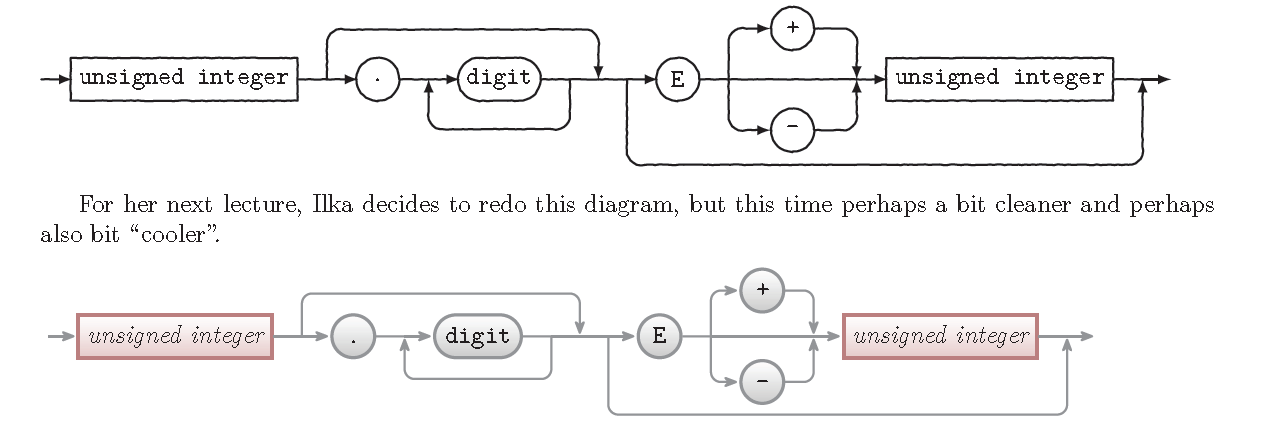
\includegraphics[width=\textwidth]{DiagramsAsSimpleGraphs.png}  % 插入图片(无需扩展名)
        \caption{这是一个示例图片}  % 图片说明
        \label{fig:example}  % 引用标签
    \end{figure}
    
\begin{tikzpicture}[
        nonterminal/.style={
            rectangle,
            minimum size=6mm,
            very thick,
            draw=red!50!black!50,
            top color=white,
            bottom color=red!50!black!20,
            font=\itshape
        }]
        \node [nonterminal] {unsigned integer};
    \end{tikzpicture}

    
\begin{tikzpicture}[node distance=5mm,
        terminal/.style={
        % The shape:
        rectangle,minimum size=6mm,rounded corners=3mm,
        % The rest
        very thick,draw=black!50,
        top color=white,bottom color=black!20,
        font=\ttfamily}]
        \node (dot) [terminal] {.};
        \node (digit) [terminal,right=of dot] {digit};
        \node (E) [terminal,right=of digit] {E};
    \end{tikzpicture}

    
\begin{tikzpicture}[node distance=5mm,
        terminal/.style={
        % The shape:
        rounded rectangle,
        minimum size=6mm,
        % The rest
        very thick,draw=black!50,
        top color=white,bottom color=black!20,
        font=\ttfamily}]
        \node (dot) [terminal] {.};
        \node (digit) [terminal,right=of dot] {digit};
        \node (E) [terminal,right=of digit] {E};
    \end{tikzpicture}

    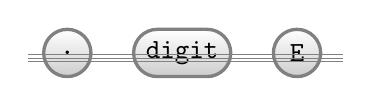
\begin{tikzpicture}[node distance=5mm]
        \node (dot) [terminal] {.};
        \node (digit) [terminal,right=of dot] {digit};
        \node (E) [terminal,right=of digit] {E};
        \draw [help lines] let \p1 = (dot.base),
        \p2 = (digit.base),
        \p3 = (E.base)
        in (-.5,\y1) -- (3.5,\y1)
        (-.5,\y2) -- (3.5,\y2)
        (-.5,\y3) -- (3.5,\y3);
    \end{tikzpicture}

    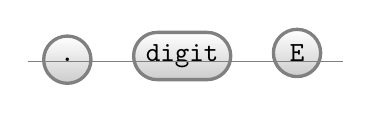
\begin{tikzpicture}[node distance=5mm]
        \node (dot) [terminal] {.};
        \node (digit) [terminal,base right=of dot] {digit};
        \node (E) [terminal,base right=of digit] {E};
        \draw [help lines] let \p1 = (dot.base),
        \p2 = (digit.base),
        \p3 = (E.base)
        in (-.5,\y1) -- (3.5,\y1)
        (-.5,\y2) -- (3.5,\y2)
        (-.5,\y3) -- (3.5,\y3);
    \end{tikzpicture}

    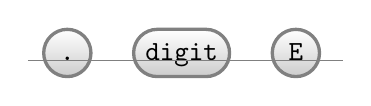
\begin{tikzpicture}[node distance=5mm,text height=1.5ex,text depth=.25ex]
        \node (dot) [terminal] {.};
        \node (digit) [terminal,base right=of dot] {digit};
        \node (E) [terminal,base right=of digit] {E};
        \draw [help lines] let \p1 = (dot.base),
        \p2 = (digit.base),
        \p3 = (E.base)
        in (-.5,\y1) -- (3.5,\y1)
        (-.5,\y2) -- (3.5,\y2)
        (-.5,\y3) -- (3.5,\y3);
    \end{tikzpicture}

    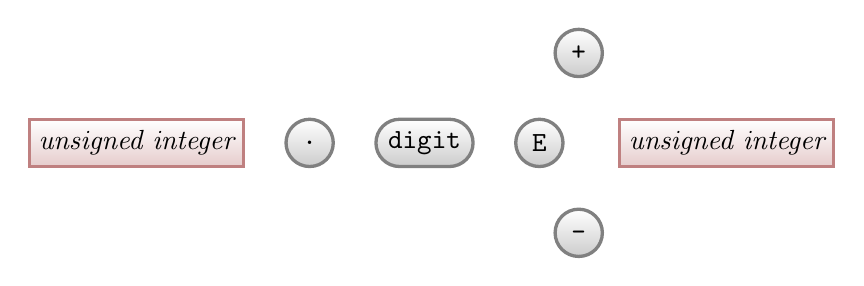
\begin{tikzpicture}[node distance=5mm and 5mm]
        \node (ui1) [nonterminal] {unsigned integer};
        \node (dot) [terminal,right=of ui1] {.};
        \node (digit) [terminal,right=of dot] {digit};
        \node (E) [terminal,right=of digit] {E};
        \node (plus) [terminal,above right=of E] {+};
        \node (minus) [terminal,below right=of E] {-};
        \node (ui2) [nonterminal,below right=of plus] {unsigned integer};
    \end{tikzpicture}

    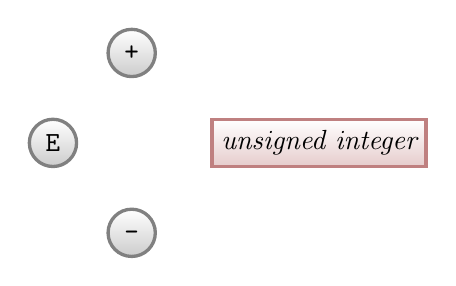
\begin{tikzpicture}[node distance=5mm and 5mm]
        \node (E) [terminal] {E};
        \node (plus) [terminal,above right=of E,xshift=5mm] {+};
        \node (minus) [terminal,below right=of E,xshift=5mm] {-};
        \node (ui2) [nonterminal,below right=of plus,xshift=5mm] {unsigned integer};
    \end{tikzpicture}

    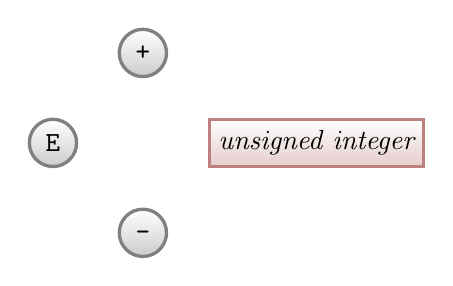
\begin{tikzpicture}[node distance=5mm and 5mm,terminal/.append style={rectangle,rounded corners=3mm}]
        \node (E) [terminal] {E};
        \node (plus) [terminal,above right=of E] {+};
        \node (minus) [terminal,below right=of E] {-};
        \node (ui2) [nonterminal,below right=of plus] {unsigned integer};
    \end{tikzpicture}

    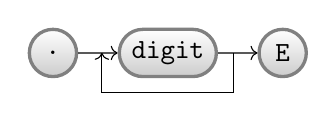
\begin{tikzpicture}[node distance=5mm and 5mm]
        \node (dot) [terminal] {.};
        \node (digit) [terminal,right=of dot] {digit};
        \node (E) [terminal,right=of digit] {E};
        \path (dot) edge[->] (digit) % simple edges
                (digit) edge[->] (E);
        \draw [->]
            % start right of digit.east, that is, at the point that is the
            % linear combination of digit.east and the vector (2mm,0pt). We
            % use the ($ ... $) notation for computing linear combinations
            ($ (digit.east) + (2mm,0) $)
            % Now go down
            -- ++(0,-.5)
            % And back to the left of digit.west
            -| ($ (digit.west) - (2mm,0) $);
    \end{tikzpicture}

    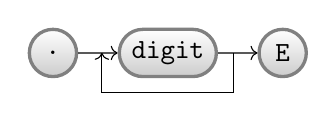
\begin{tikzpicture}[node distance=5mm and 5mm,
        skip loop/.style={to path={-- ++(0,-.5) -| (\tikztotarget)}}]
        \node (dot) [terminal] {.};
        \node (digit) [terminal,right=of dot] {digit};
        \node (E) [terminal,right=of digit] {E};
        \path (dot) edge[->] (digit) % simple edges
                (digit) edge[->] (E)
        ($ (digit.east) + (2mm,0) $)
        edge[->,skip loop] ($ (digit.west) - (2mm,0) $);
    \end{tikzpicture}

    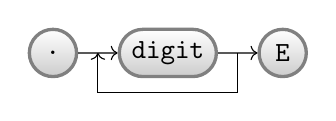
\begin{tikzpicture}[node distance=5mm and 5mm,
        skip loop/.style={to path={-- ++(0,#1) -| (\tikztotarget)}}]
        \node (dot) [terminal] {.};
        \node (digit) [terminal,right=of dot] {digit};
        \node (E) [terminal,right=of digit] {E};
        \path (dot) edge[->] (digit) % simple edges
        (digit) edge[->] (E)
        ($ (digit.east)!.5!(E.west) $)
        edge[->,skip loop=-5mm] ($ (digit.west)!.5!(dot.east) $);
    \end{tikzpicture}

    
\begin{tikzpicture}
        \matrix[row sep=1mm,column sep=5mm] {
        % First row:
        & & & & \node [terminal] {+}; & \\
        % Second row:
        \node [nonterminal] {unsigned integer}; &
        \node [terminal] {.}; &
        \node [terminal] {digit}; &
        \node [terminal] {E}; &&
        \node [nonterminal] {unsigned integer}; \\
        % Third row:
        & & & & \node [terminal] {-}; & \\
        };
    \end{tikzpicture}

    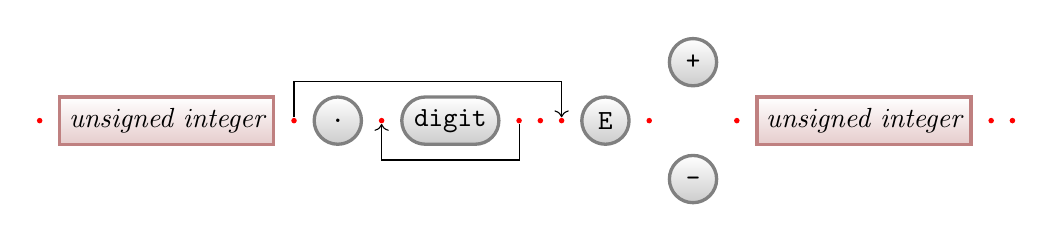
\begin{tikzpicture}[point/.style={circle,inner sep=0pt,minimum size=2pt,fill=red},
        skip loop/.style={to path={-- ++(0,#1) -| (\tikztotarget)}}]
        \matrix[row sep=1mm,column sep=2mm] {
        % First row:
        & & & & & & & & & & & \node (plus) [terminal] {+};\\
        % Second row:
        \node (p1) [point] {}; & \node (ui1) [nonterminal] {unsigned integer}; &
        \node (p2) [point] {}; & \node (dot) [terminal] {.}; &
        \node (p3) [point] {}; & \node (digit) [terminal] {digit}; &
        \node (p4) [point] {}; & \node (p5) [point] {}; &
        \node (p6) [point] {}; & \node (e) [terminal] {E}; &
        \node (p7) [point] {}; & &
        \node (p8) [point] {}; & \node (ui2) [nonterminal] {unsigned integer}; &
        \node (p9) [point] {}; & \node (p10) [point] {};\\
        % Third row:
        & & & & & & & & & & & \node (minus)[terminal] {-};\\
        };
        \path (p4) edge [->,skip loop=-5mm] (p3)
        (p2) edge [->,skip loop=5mm] (p6);
    \end{tikzpicture}

    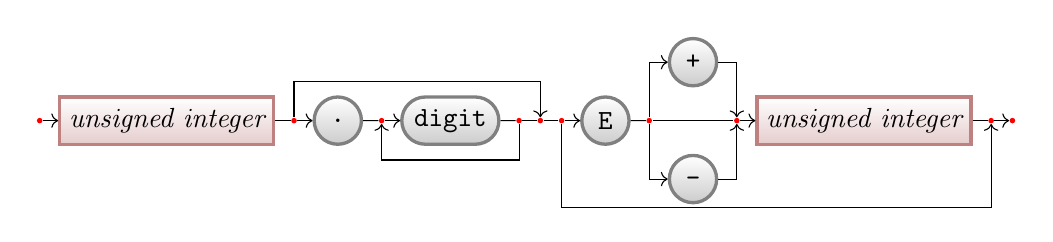
\begin{tikzpicture}[
        point/.style={circle,inner sep=0pt,minimum size=2pt,fill=red},
        skip loop/.style={to path={-- ++(0,#1) -| (\tikztotarget)}},
        hv path/.style={to path={-| (\tikztotarget)}},
        vh path/.style={to path={|- (\tikztotarget)}}]
        \matrix[row sep=1mm,column sep=2mm] {
            % First row:
            & & & & & & & & & & & \node (plus) [terminal] {+};\\
            % Second row:
            \node (p1) [point] {}; & \node (ui1) [nonterminal] {unsigned integer}; &
            \node (p2) [point] {}; & \node (dot) [terminal] {.}; &
            \node (p3) [point] {}; & \node (digit) [terminal] {digit}; &
            \node (p4) [point] {}; & \node (p5) [point] {}; &
            \node (p6) [point] {}; & \node (e) [terminal] {E}; &
            \node (p7) [point] {}; & &
            \node (p8) [point] {}; & \node (ui2) [nonterminal] {unsigned integer}; &
            \node (p9) [point] {}; & \node (p10) [point] {};\\
            % Third row:
            & & & & & & & & & & & \node (minus)[terminal] {-};\\
        };


        \graph {
            (p1) -> (ui1) -- (p2) -> (dot) -- (p3) -> (digit) -- (p4)
            -- (p5) -- (p6) -> (e) -- (p7) -- (p8) -> (ui2) -- (p9) -> (p10);
            (p4) ->[skip loop=-5mm] (p3);
            (p2) ->[skip loop=5mm] (p5);
            (p6) ->[skip loop=-11mm] (p9);
            (p7) ->[vh path] (plus) -> [hv path] (p8);
            (p7) ->[vh path] (minus) -> [hv path] (p8);
        };
    \end{tikzpicture}

    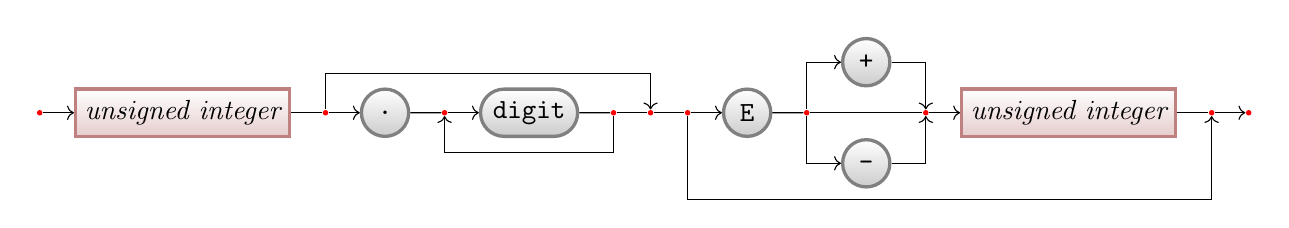
\begin{tikzpicture}[
        point/.style={circle,inner sep=0pt,minimum size=2pt,fill=red},
        skip loop/.style={to path={-- ++(0,#1) -| (\tikztotarget)}},
        hv path/.style={to path={-| (\tikztotarget)}},
        vh path/.style={to path={|- (\tikztotarget)}}]
        \matrix[column sep=4mm] {
            % First row:
            & & & & & & & & & & & \node (plus) [terminal] {+};\\
            % Second row:
            \node (p1) [point] {}; & \node (ui1) [nonterminal] {unsigned integer}; &
            \node (p2) [point] {}; & \node (dot) [terminal] {.}; &
            \node (p3) [point] {}; & \node (digit) [terminal] {digit}; &
            \node (p4) [point] {}; & \node (p5) [point] {}; &
            \node (p6) [point] {}; & \node (e) [terminal] {E}; &
            \node (p7) [point] {}; & &
            \node (p8) [point] {}; & \node (ui2) [nonterminal] {unsigned integer}; &
            \node (p9) [point] {}; & \node (p10) [point] {};\\
            % Third row:
            & & & & & & & & & & & \node (minus)[terminal] {-};\\
        };


        \graph {
            (p1) -> (ui1) -- (p2) -> (dot) -- (p3) -> (digit) -- (p4)
            -- (p5) -- (p6) -> (e) -- (p7) -- (p8) -> (ui2) -- (p9) -> (p10);
            (p4) ->[skip loop=-5mm] (p3);
            (p2) ->[skip loop=5mm] (p5);
            (p6) ->[skip loop=-11mm] (p9);
            (p7) ->[vh path] (plus) -> [hv path] (p8);
            (p7) ->[vh path] (minus) -> [hv path] (p8);
        };
    \end{tikzpicture}


    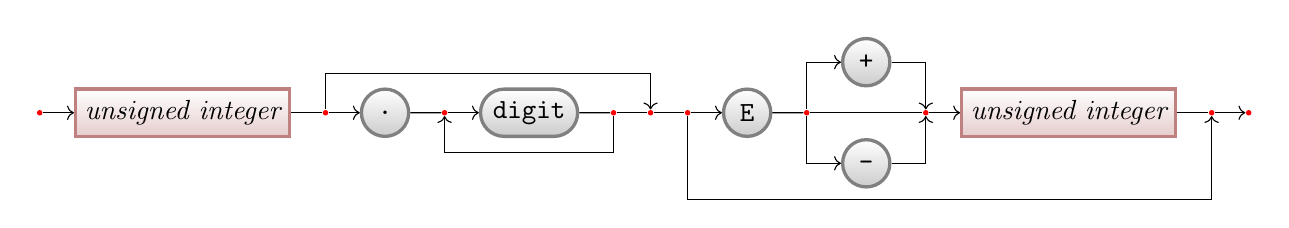
\begin{tikzpicture}[
        point/.style={circle,inner sep=0pt,minimum size=2pt,fill=red},
        skip loop/.style={to path={-- ++(0,#1) -| (\tikztotarget)}},
        hv path/.style={to path={-| (\tikztotarget)}},
        vh path/.style={to path={|- (\tikztotarget)}}]
        \matrix[column sep=4mm] {
            % First row:
            & & & & & & & & & & & \node (plus) [terminal] {+};\\
            % Second row:
            \node (p1) [point] {}; & \node (ui1) [nonterminal] {unsigned integer}; &
            \node (p2) [point] {}; & \node (dot) [terminal] {.}; &
            \node (p3) [point] {}; & \node (digit) [terminal] {digit}; &
            \node (p4) [point] {}; & \node (p5) [point] {}; &
            \node (p6) [point] {}; & \node (e) [terminal] {E}; &
            \node (p7) [point] {}; & &
            \node (p8) [point] {}; & \node (ui2) [nonterminal] {unsigned integer}; &
            \node (p9) [point] {}; & \node (p10) [point] {};\\
            % Third row:
            & & & & & & & & & & & \node (minus)[terminal] {-};\\
        };


        \graph[use existing nodes] {
            p1 -> ui1 -- p2 -> dot -- p3 -> digit -- p4 -- p5 -- p6 -> e -- p7 -- p8 -> ui2 -- p9 -> p10;
            p4 ->[skip loop=-5mm] p3;
            p2 ->[skip loop=5mm] p5;
            p6 ->[skip loop=-11mm] p9;
            p7 ->[vh path] { plus, minus } -> [hv path] p8;
        };
    \end{tikzpicture}

    \tikz \graph [grow right=2cm] { unsigned integer -> d -> digit -> E };

    \tikz \graph [grow right sep] {
        unsigned integer[nonterminal] -> "."[terminal] -> digit[terminal] -> E[terminal]
    };

    \tikz \graph [grow right sep] {
        unsigned integer [nonterminal] ->
        "." [terminal] ->
        digit [terminal] ->
        E [terminal] ->
        {
            "+" [terminal],
            "" [coordinate],
            "-" [terminal]
        } ->
        ui2/unsigned integer [nonterminal]
    };

    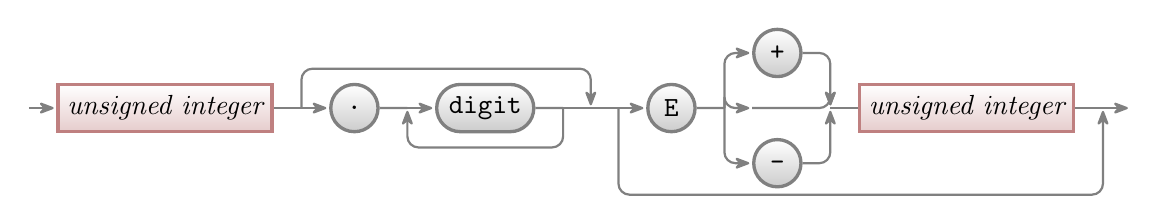
\begin{tikzpicture}[>={Stealth[round]}, thick, black!50, text=black,
        every new ->/.style={shorten >=1pt},
        graphs/every graph/.style={edges=rounded corners}]
        \graph [grow right sep, branch down=7mm] {
        / [coordinate] ->
        unsigned integer [nonterminal] --
        p1 [coordinate] ->
        "." [terminal] --
        p2 [coordinate] ->
        digit [terminal] --
        p3 [coordinate] --
        p4 [coordinate] --
        p5 [coordinate] ->
        E [terminal] --
        q1 [coordinate] ->[vh path]
        { [nodes={yshift=7mm}]
            "+" [terminal],
            q2/ [coordinate],
            "-" [terminal]
        } -> [hv path]
        q3 [coordinate] --
        /unsigned integer [nonterminal] --
        p6 [coordinate] ->
        / [coordinate];
        p1 ->[skip loop=5mm] p4;
        p3 ->[skip loop=-5mm] p2;
        p5 ->[skip loop=-11mm] p6;
        };
    \end{tikzpicture}

    \tikz \graph [grow right sep, left anchor=east, right anchor=west] {
                    start -- {
                    long text -- {short, very long text} -- more text,
                    long -- longer -- longest
                    } -- end
                };

    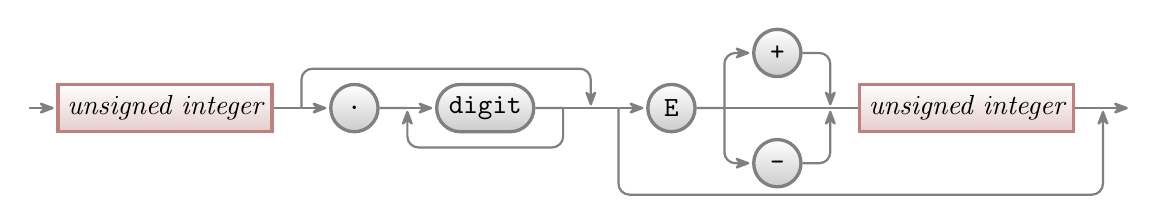
\begin{tikzpicture}[>={Stealth[round]}, thick, black!50, text=black,
        every new ->/.style={shorten >=1pt},
        graphs/every graph/.style={edges=rounded corners}]
        \graph [grow right sep, branch down=7mm,simple] {
            / [coordinate] ->
            unsigned integer [nonterminal] --
            p1 [coordinate] ->
            "." [terminal] --
            p2 [coordinate] ->
            digit [terminal] --
            p3 [coordinate] --
            p4 [coordinate] --
            p5 [coordinate] ->
            E [terminal] --
            q1 [coordinate] ->[vh path]
            { [nodes={yshift=7mm}]
                "+" [terminal],
                q2/ [coordinate],
                "-" [terminal]
            } -> [hv path]
            q3 [coordinate] --
            /unsigned integer [nonterminal] --
            p6 [coordinate] ->
            / [coordinate];


            p1 ->[skip loop=5mm] p4;
            p3 ->[skip loop=-5mm] p2;
            p5 ->[skip loop=-11mm] p6;

            q1 -- q2 -- q3; % make these edges plain
        };

        
    \end{tikzpicture}
\end{document}